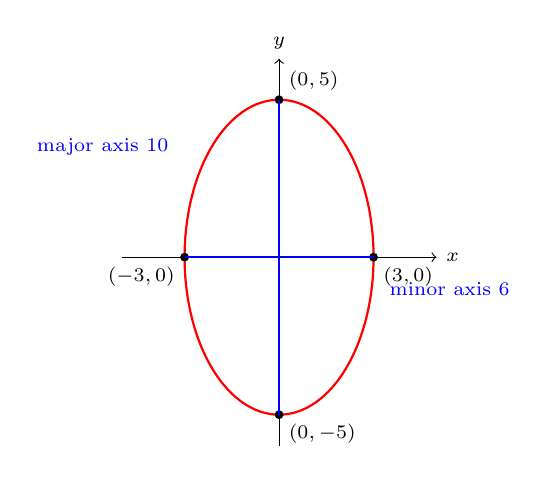
\begin{tikzpicture}[scale=0.4, every node/.style={font=\scriptsize}]
  \draw[->] (-5,0) -- (5,0) node[right] {$x$};
  \draw[->] (0,-6) -- (0,6.3) node[above] {$y$};
  \draw[red, thick] (0,0) ellipse (3 and 5);
  \fill (0,5) circle (4pt) node[above right] {$(0,5)$};
  \fill (0,-5) circle (4pt) node[below right] {$(0,-5)$};
  \fill (3,0) circle (4pt) node[below right] {$(3,0)$};
  \fill (-3,0) circle (4pt) node[below left] {$(-3,0)$};
  \draw[blue, thick] (-3,0) -- (3,0);
  \draw[blue, thick] (0,-5) -- (0,5);
  \node[blue, left] at (-3.2,3.5) {major axis $10$};
  \node[blue, right] at (3.2,-1) {minor axis $6$};
\end{tikzpicture}
